\documentclass{article}

\usepackage{geometry}
 \geometry{
 a4paper,
 total={170mm,257mm},
 left=20mm,
 top=20mm,
 }

\setlength{\parskip}{7pt}
\setlength{\parindent}{0pt}

\title{Using the Diligent JTAG-HS2 Programming Cable with OpenOCD}
\date{2019-10-11}

\PassOptionsToPackage{hyphens}{url}\usepackage{hyperref}
\usepackage{listings}
\usepackage{amssymb}
\usepackage{graphicx}
\graphicspath{ {./images/} }
\usepackage{float}

\lstset{
	breaklines=true,
	frame=single
}

\begin{document}
	\maketitle
	
	\section{About}
	
	The JTAG-HS2 Programming Cable is an USB JTAG probe. It is available here: \url{https://store.digilentinc.com/jtag-hs2-programming-cable/}
	
	\begin{figure}[H]
   	\centering
   	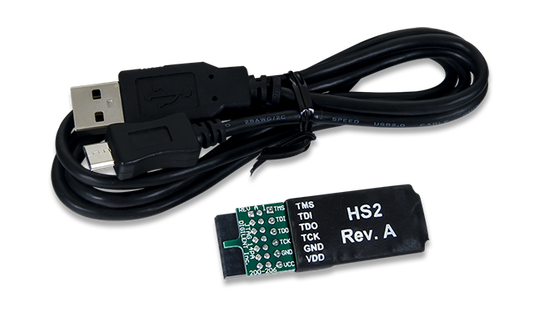
\includegraphics[width=0.6\textwidth]{hs2.png}
	\end{figure}
	
	The cable is fully compatible with all Xilinx tools, but it can also be used with OpenOCD.
	
	\section{Software configuration}
	
	\subsection{Libusb}
	
	You need libusb to use the cable.
	
	On Ubuntu, you can use apt:
	
	\begin{lstlisting}[language=bash]
    $ sudo apt install libusb-1.0-0-dev
    \end{lstlisting}
    
    You can also build it yourself using the sources available on \url{https://libusb.info}
    
    \subsection{Libftdi}
    
    The cable contains an FTDI chip, so you need libftdi.
    
    Ubuntu:
    
    \begin{lstlisting}[language=bash]
    $ sudo apt install libftdi1-dev
    \end{lstlisting}
    
    Or from sources: \url{https://www.intra2net.com/en/developer/libftdi/download.php}
    
    \subsection{OpenOCD Compilation}
    
    The OpenOCD interface used with the cable is \textit{ftdi}.
    
    To enable this interface, use the \textit{-{}-enable-ftdi} option when compiling OpenOCD.
    
    \begin{lstlisting}[language=bash]
    $ ./configure --enable-ftdi <other options>
    \end{lstlisting}
    
    If you are not sure if your existing instance of OpenOCD supports the ftdi interface, you can list the debug adapter drivers that have been built into the running copy of OpenOCD with:
    
    \begin{lstlisting}[language=bash]
    $ openocd -c interface_list
    \end{lstlisting}
    
    \subsection{udev rules}
    
    It is necessary to add a udev rule to use the cable.
    
    OpenOCD provides a file containing the rule we need. Copy it into /etc/udev/rules.d/
    
    \begin{lstlisting}[language=bash]
    $ sudo cp <openocd>/contrib/60-openocd.rules /etc/udev/rules.d
    \end{lstlisting}
    
    The file is also available here: \url{https://github.com/riscv/riscv-openocd/blob/riscv/contrib/60-openocd.rules}
    
    The particular entry about the HS2 cable is :
    
    \begin{lstlisting}
    ATTRS{idVendor}=="0403", ATTRS{idProduct}=="6014", MODE="660", GROUP="plugdev", TAG+="uaccess"
    \end{lstlisting}
    
    The either reboot your system or reload the udev configuration with :
    
    \begin{lstlisting}[language=bash]
    $ sudo udevadm control --reload
    \end{lstlisting}
    
    \subsection{Checking}
    
    To check if the cable is recognized, run lsusb. There should be a line like this:
    
    \begin{lstlisting}[language=bash]
    $ lsusb
    [...]
    Bus 005 Device 003: ID 0403:6014 Future Technology Devices International, Ltd FT232H Single HS USB-UART/FIFO IC
    [...]
    \end{lstlisting}
    
    For more details about the device, use more options:
    
    \begin{lstlisting}[language=bash]
    $ lsusb -v -d 0403:6014
    \end{lstlisting}
    
    \newpage
    \section{OpenOCD Config File}
    
    Examples of config files using the HS2 cable are:
    
    \vspace{-\topsep}
	\begin{itemize}
	\item \url{https://github.com/pulp-platform/pulpissimo/blob/master/fpga/pulpissimo-zedboard/openocd-zedboard-hs2.cfg}
	\item \url{https://github.com/arduino/OpenOCD/blob/master/tcl/interface/ftdi/digilent-hs2.cfg}
	\end{itemize}
	
	Generally, for the interface part of the config file, you can use:
	
	\begin{lstlisting}
interface ftdi
ftdi_device_desc "Digilent USB Device"
ftdi_vid_pid 0x0403 0x6014
ftdi_serial 210249A85F9B
ftdi_channel 0						
ftdi_layout_init 0x00e8 0x60eb

reset_config none
    \end{lstlisting}
    
    Use \textbf{lsusb -v -d 0403:6014} to find the necessary values :
    
    \vspace{-\topsep}
	\begin{itemize}
	\item \textbf{ftdi\_device\_desc}: this command should use the same value as the \textbf{iProduct} field
	
	\item \textbf{ftdi\_vid\_pid}: \textbf{idVendor} and \textbf{idProduct}
	
	\item \textbf{ftdi\_serial}: this command is useful if there are more than one adapter connected to the host and can be omitted otherwise. The needed value is in the \textbf{iSerial} field.
	
	\item \textbf{ftdi\_channel}: the default (channel 0) is fine
	
	\item \textbf{ftdi\_layout\_init}: initial values of the FTDI GPIO data and direction registers. Refer to the adapter schematics to find them. 0x00e8 and 0x60eb work for the HS2 cable
	\end{itemize}
	
	For more information about the OpenOCD commands, see \url{http://www.openocd.org/doc/html/Debug-Adapter-Configuration.html}
	
	\section{Hardware configuration}
	
	The HS2 cable does not use the TRST signal. 
	
	Do not leave the pin floating and tie it to 1 if the target TAP reset is active low, or 0 if it is active high.
	
	\section{Vivado Hardware Manager}
	
	
	
\end{document}